\section{Amministratore}
\subsection{UC5.1 Approvazione registrazione}

\begin{figure}[H]
\centering
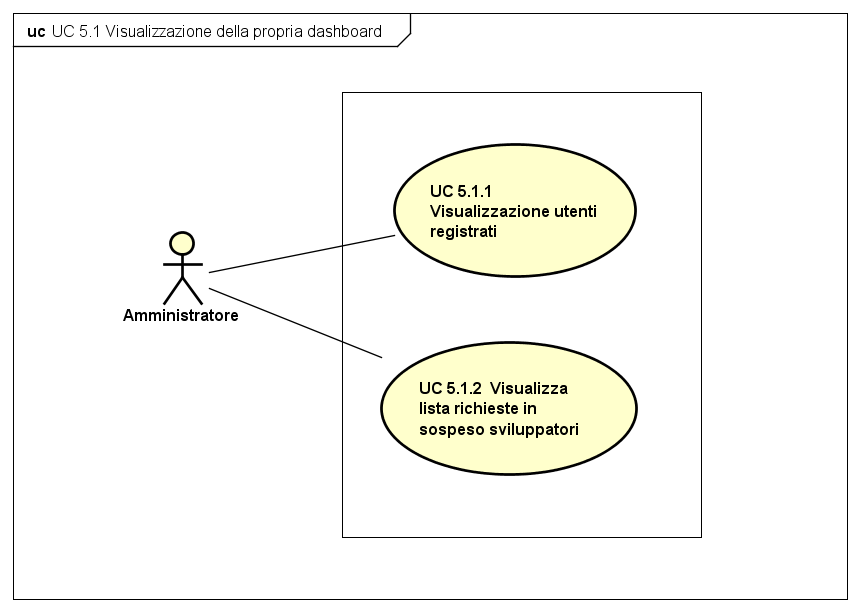
\includegraphics[width=10cm,height=9cm]{img/UC51.png} 
\caption{Caso d'uso UC5.1}
\end{figure}

\begin{itemize}
\item[•] \textbf{Attore}: Amministratore;

\item[•] \textbf{Descrizione}: L’amministratore approva la richiesta di registrazione da parte dello sviluppatore;

\item[•] \textbf{Precondizione}: Lo sviluppatore ha effettuato richiesta di registrazione, l'amministratore visualizza le richieste di registrazione da parte degli sviluppatori che desiderano accedere ai dati della piattaforma;

\item[•] \textbf{Postcondizione}: L’amministratore approva lo sviluppatore;

\item[•] \textbf{Flusso degli eventi}:

\begin{enumerate}

\item Visualizzazione elenco richieste;

\item Selezione richiesta sviluppatore;

\item Approvazione utenza sviluppatore.

\end{enumerate}

\end{itemize}


\subsection{UC5.2 Rifiuto registrazione}

\begin{figure}[H]
\centering
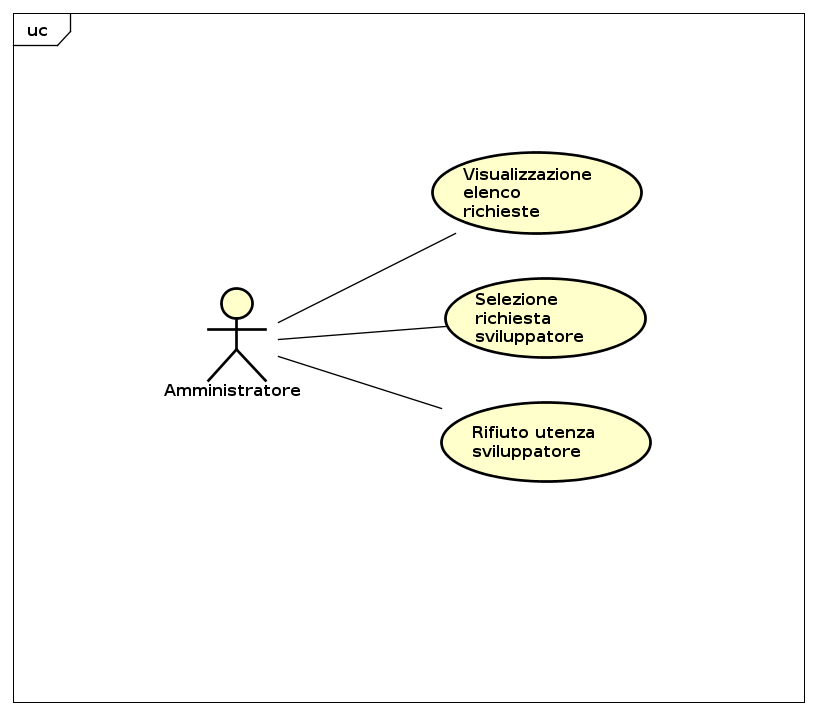
\includegraphics[width=11cm]{img/UC52.png} 
\caption{Caso d'uso UC5.2}
\end{figure}


\begin{itemize}
\item[•] \textbf{Attore}: Amministratore;

\item[•] \textbf{Descrizione}: L’amministratore rifiuta la richiesta di registrazione da parte dello sviluppatore;

\item[•] \textbf{Precondizione}: Lo sviluppatore ha richiesto l’approvazione, l’amministratore visualizza la richiesta di registrazione da parte dello sviluppatore che desidera accedere ai dati della piattaforma;

\item[•] \textbf{Postcondizione}: L’amministratore rifiuta la richiesta di registrazione dello sviluppatore;

\item[•] \textbf{Flusso degli eventi}:

\begin{enumerate}

\item Visualizzazione elenco richieste;

\item Selezione richiesta sviluppatore;

\item Rifiuto utenza sviluppatore.

\end{enumerate}
\end{itemize}
\subsection{UC5.3 Eliminazione utenza}


\begin{figure}[H]
\centering
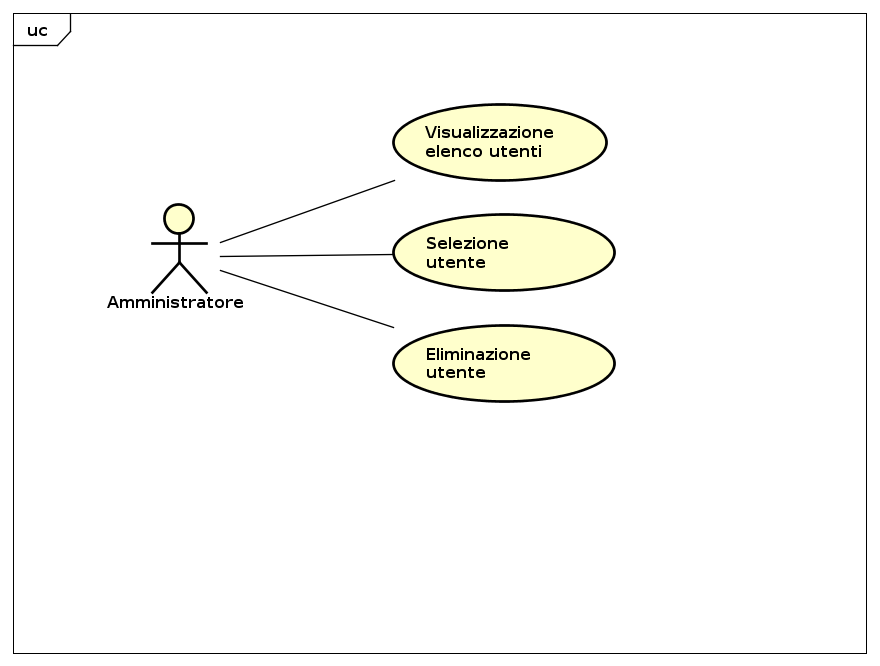
\includegraphics[width=11cm]{img/UC53.png} 
\caption{Caso d'uso UC5.3}
\end{figure}


\begin{itemize}
\item[•] \textbf{Attore}: Amministratore;

\item[•] \textbf{Descrizione}: L’amministratore elimina un’utenza dal sistema;

\item[•] \textbf{Precondizione}: L’amministratore \`{e} autenticato e visualizza l’elenco degli utenti nel sistema, e l’utenza da eliminare \`{e} registrata nel sistema;

\item[•] \textbf{Postcondizione}: L’amministratore ha eliminato l’utenza dal sistema; 

\item[•] \textbf{Flusso degli eventi}:

\begin{enumerate}

\item Visualizzazione elenco utenti;

\item Selezione utente;

\item Eliminazione utente.

\end{enumerate}

\end{itemize}
